\documentclass[journal,12pt,twocolumn]{IEEEtran}

\usepackage{setspace}
\usepackage{gensymb}

\singlespacing


\usepackage[cmex10]{amsmath}

\usepackage{amsthm}

\usepackage{mathrsfs}
\usepackage{txfonts}
\usepackage{stfloats}
\usepackage{bm}
\usepackage{cite}
\usepackage{cases}
\usepackage{subfig}
 
\usepackage{longtable}
\usepackage{multirow}

\usepackage{enumitem}
\usepackage{mathtools}
\usepackage{steinmetz}
\usepackage{tikz}
\usepackage{circuitikz}
\usepackage{verbatim}
\usepackage{tfrupee}
\usepackage[breaklinks=true]{hyperref}
\usepackage{graphicx}
\usepackage{tkz-euclide}
\usepackage{amsmath}

\usetikzlibrary{calc,math}
\usepackage{listings}
    \usepackage{color}                                            %%
    \usepackage{array}                                            %%
    \usepackage{longtable}                                        %%
    \usepackage{calc}                                             %%
    \usepackage{multirow}                                         %%
    \usepackage{hhline}                                           %%
    \usepackage{ifthen}                                           %%
    \usepackage{lscape}     
\usepackage{multicol}
\usepackage{chngcntr}

\DeclareMathOperator*{\Res}{Res}

\renewcommand\thesection{\arabic{section}}
\renewcommand\thesubsection{\thesection.\arabic{subsection}}
\renewcommand\thesubsubsection{\thesubsection.\arabic{subsubsection}}

\renewcommand\thesectiondis{\arabic{section}}
\renewcommand\thesubsectiondis{\thesectiondis.\arabic{subsection}}
\renewcommand\thesubsubsectiondis{\thesubsectiondis.\arabic{subsubsection}}



\def\inputGnumericTable{}                                 %%

\lstset{
%language=C,
frame=single, 
breaklines=true,
columns=fullflexible
}
\begin{document}


\newtheorem{theorem}{Theorem}[section]
\newtheorem{problem}{Problem}
\newtheorem{proposition}{Proposition}[section]
\newtheorem{lemma}{Lemma}[section]
\newtheorem{corollary}[theorem]{Corollary}
\newtheorem{example}{Example}[section]
\newtheorem{definition}[problem]{Definition}

\newcommand{\BEQA}{\begin{eqnarray}}
\newcommand{\EEQA}{\end{eqnarray}}
\newcommand{\define}{\stackrel{\triangle}{=}}
\bibliographystyle{IEEEtran}
\providecommand{\mbf}{\mathbf}
\providecommand{\pr}[1]{\ensuremath{\Pr\left(#1\right)}}
\providecommand{\qfunc}[1]{\ensuremath{Q\left(#1\right)}}
\providecommand{\sbrak}[1]{\ensuremath{{}\left[#1\right]}}
\providecommand{\lsbrak}[1]{\ensuremath{{}\left[#1\right.}}
\providecommand{\rsbrak}[1]{\ensuremath{{}\left.#1\right]}}
\providecommand{\brak}[1]{\ensuremath{\left(#1\right)}}
\providecommand{\lbrak}[1]{\ensuremath{\left(#1\right.}}
\providecommand{\rbrak}[1]{\ensuremath{\left.#1\right)}}
\providecommand{\cbrak}[1]{\ensuremath{\left\{#1\right\}}}
\providecommand{\lcbrak}[1]{\ensuremath{\left\{#1\right.}}
\providecommand{\rcbrak}[1]{\ensuremath{\left.#1\right\}}}
\theoremstyle{remark}
\newtheorem{rem}{Remark}
\newcommand{\sgn}{\mathop{\mathrm{sgn}}}
\providecommand{\abs}[1]{\l\vert#1\r\vert}
\providecommand{\res}[1]{\Res\displaylimits_{#1}} 
\providecommand{\norm}[1]{\lVert#1\rVert}
%\providecommand{\norm}[1]{\lVert#1\rVert}
\providecommand{\mtx}[1]{\mathbf{#1}}
\providecommand{\mean}[1]{E\l[ #1 \r]}
\providecommand{\fourier}{\overset{\mathcal{F}}{ \rightleftharpoons}}
%\providecommand{\hilbert}{\overset{\mathcal{H}}{ \rightleftharpoons}}
\providecommand{\system}{\overset{\mathcal{H}}{ \longleftrightarrow}}
	%\newcommand{\solution}[2]{\textbf{Solution:}{#1}}
\newcommand{\solution}{\noindent \textbf{Solution: }}
\newcommand{\cosec}{\,\text{cosec}\,}
\providecommand{\dec}[2]{\ensuremath{\overset{#1}{\underset{#2}{\gtrless}}}}
\newcommand{\myvec}[1]{\ensuremath{\begin{pmatrix}#1\end{pmatrix}}}
\newcommand{\mydet}[1]{\ensuremath{\begin{vmatrix}#1\end{vmatrix}}}
\numberwithin{equation}{subsection}
\makeatletter
\@addtoreset{figure}{problem}
\makeatother
\let\StandardTheFigure\thefigure
\let\vec\mathbf
\renewcommand{\thefigure}{\theproblem}
\def\putbox#1#2#3{\makebox[0in][l]{\makebox[#1][l]{}\raisebox{\baselineskip}[0in][0in]{\raisebox{#2}[0in][0in]{#3}}}}
     \def\rightbox#1{\makebox[0in][r]{#1}}
     \def\centbox#1{\makebox[0in]{#1}}
     \def\topbox#1{\raisebox{-\baselineskip}[0in][0in]{#1}}
     \def\midbox#1{\raisebox{-0.5\baselineskip}[0in][0in]{#1}}
\vspace{3cm}
\title{Assignment 3}
\author{Kavya Kamal}
\maketitle
\newpage
\bigskip
\renewcommand{\thefigure}{\theenumi}
\renewcommand{\thetable}{\theenumi}
Download all python codes from 
\begin{lstlisting}
https://github.com/kavyakamal66/IITH-INTERNSHIP/blob/main/Assignment3/code3.py
\end{lstlisting}

%
and latex-tikz codes from 
%
\begin{lstlisting}
https://github.com/kavyakamal66/IITH-INTERNSHIP/blob/main/Assignment3/assignment3.tex
\end{lstlisting}

\section{\textbf{Question No. 2.1 - Quadratic forms}}

\noindent Find the equation of circle passing through $\myvec{0\\0}$ making intercepts $a$ and $b$ on the co-ordinate axis.
%

\section{\textbf {Solution}}


The general equation of circle is,

\begin{equation}
\vec{x^\top}\vec{x}+2\vec{u^\top}\vec{x}+f=0 
\end{equation}
Since the circle passes through $\myvec{0\\0}$, the equation of given circle is,
\begin{equation}
    \vec{x^\top}\vec{x}+2\vec{u^\top}\vec{x}=0 \label{eq:0}
\end{equation}

Given intercepts are $\myvec{a\\0}$ and $\myvec{0\\b}$ \\
\begin{figure}[!h]
         \centering
         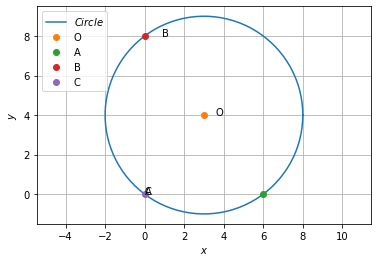
\includegraphics[width=\columnwidth]{figure3.png}
         \caption{Plot of the required circle}
         \label{Figure}
\end{figure}\\

Let 
\begin{equation}
 \vec{A}=\myvec{a\\0} ,\\
 \vec{B}=\myvec{b\\0},\\
 \vec{C}=\myvec{0\\0}
\end{equation}
Substituting the given co-ordinates,\\
Equation of circle from \eqref{eq:0},
\begin{equation}
    \vec{A^\top}\vec{A}+2\vec{u^\top}\vec{A}=0 \label{eq:4}
\end{equation}
\begin{equation}
    \vec{B^\top}\vec{B}+2\vec{u^\top}\vec{B}=0 \label{eq:5}
\end{equation}
Simplifying \eqref{eq:4} and \eqref{eq:5}
\begin{equation}
    \myvec{a & 0 \\ 0 & b}\vec{u^\top}= \myvec{-a^2/2 \\ -b^2/2}
\end{equation}

\begin{equation}
\implies \myvec{a & 0 & -a^2/2 \\ 0 & b & -b^2/2}
\xleftrightarrow [R_1\leftarrow R_1/a]{R_2\leftarrow R_2/b}
\end{equation}

\begin{equation}
  \implies \myvec{1 & 0 & -a/2 \\ 0& 1 & -b/2}
\end{equation}


\begin{equation}
    \implies \vec{u}=\myvec{-a/2 & -b/2} 
\end{equation}

\begin{equation}
    \vec{u} = \vec{-O}
\end{equation}

\begin{equation}
    \vec{O} = \myvec{a/2 & b/2}
\end{equation}
Substituting this in \eqref{eq:0},
\begin{equation}
    \vec{x^\top}\vec{x}+2\myvec{-a/2 \\ -b/2}\vec{x}=0 
\end{equation}
\begin{equation}
   \implies \vec{x^\top}\vec{x}-\myvec{a \\ b }\vec{x}=0
\end{equation}
Substituting, $a=6$ and $b=8$,the circle is plotted.
Equation of given circle is,
\begin{equation}
   \implies \vec{x^\top}\vec{x}-\myvec{6 \\ 8 }\vec{x}=0
\end{equation}


\end{document}
